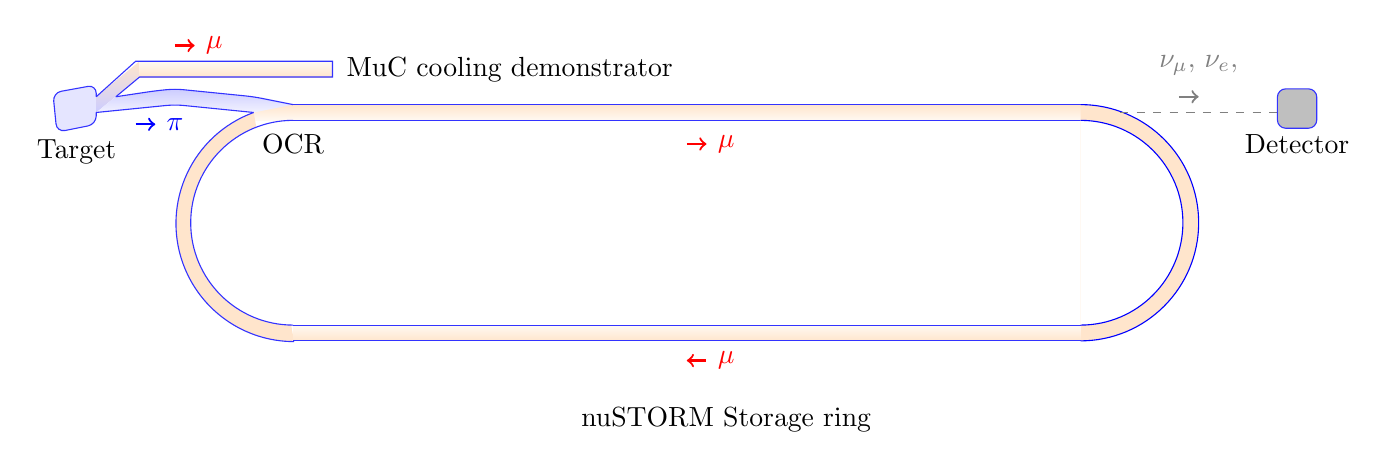
\begin{tikzpicture}[scale=0.05]
% target
\draw[blue!80, rounded corners=3pt, fill=blue!10] (10,-2) -- (10,-5) -- (0,-7) -- (-1,3) -- (10,5) -- (10, 2);
\node[] at (5,-12) {Target};


%Demo
\shade[bottom color=blue!20,top color=orange!20] (10,-2) -- (21,7) -- (21,11) -- (10,2);
\shade[bottom color=orange!20,top color=orange!5] (70,11) -- (70,7) -- (21, 7) -- (21, 11);
\draw[blue!80] (10,2) -- (20,11) -- (70,11) -- (70,7) -- (21, 7) -- (15, 2);
\node[] at (115,9) {MuC cooling demonstrator};
\draw[thick,->, color=red] (30,15) -- (35,15);
\node[text=red] at (40,15) {$\mu$};

% storage ring
\shade[top color=orange!20, bottom color=orange!5] (50, 0) -- (260,0) -- (260,-4) -- (50, -4);
\draw[blue!80, fill=orange!20] (50,-2) arc (110:270:30);
\draw[blue!80, fill=white] (60,-4) arc (90:270:26);
\draw[blue!80] (60, 0) -- (260,0);
\draw[blue!80] (60, -4) -- (260,-4);
\draw[blue, fill=orange!20] (260,-60) arc (-90:90:30);
\draw[blue, fill=white] (260,-56) arc (-90:90:26);
\shade[top color=orange!5, bottom color=orange!20] (60, -56) -- (260,-56) -- (260,-60) -- (60, -60);
\draw[blue!80] (60, -56) -- (260,-56);
\draw[blue!80] (60, -60) -- (260,-60);
\draw[thick,->, color=red] (160,-10) -- (165,-10);
\node[text=red] at (170,-10) {$\mu$};
\draw[thick,<-, color=red] (160,-65) -- (165,-65);
\node[text=red] at (170,-65) {$\mu$};
\node[] at (170,-80) {nuSTORM Storage ring};

%Pion line
\shade[bottom color=blue!5,top color=blue!20] (15, 2) -- (25,3.5) -- (30,4) -- (35,3.5) -- (50,2) -- (60,0) -- (50,-2) -- (35,-0.5) -- (30,0) -- (25,-0.5) -- (10, -2);
\draw[blue!80, rounded corners=3pt] (15, 2) -- (25,3.5) -- (30,4) -- (35,3.5) -- (50,2) -- (60,0);
\draw[blue!80, rounded corners=3pt] (10, -2) -- (25,-0.5) -- (30,0) -- (35,-0.5) -- (50,-2);
\draw[thick,->, color=blue] (20,-5) -- (25,-5);
\node[text=blue] at (30,-5) {$\pi$};
\node[] at (60,-10) {OCR};


% detector
\draw[gray, dashed] (270,-2) -- (310, -2);
\draw[blue!80, fill=gray!50, rounded corners=3pt] (310,-6) rectangle (320,4);
\draw[thick,->, color=gray] (285,2) -- (290,2);
\node[text=gray] at (290,10) {$\nu_{\mu}$, $\nu_{e}$, };
\node[] at (315,-10) {Detector};

\end{tikzpicture}
